\documentclass{article}

\usepackage[margin=1in]{geometry}
\usepackage{amsmath,amssymb}
\usepackage{lscape}
\usepackage{graphicx}


\begin{document}

\title{Autonomous Agents Report\\Assignment 1: Single Agent Planning}
\author{Agnes van Belle (10363130), \\Maaike Fleuren (10350470), \\Norbert Heijne (10357769), \\Lydia Mennes (10333843)}
\maketitle

This report has been written for the Master Artificial Intelligence course Autonomous Agents. The assignments that will be worked out in detail in this report include the following topics: "Single Agent Planning, Single Agent Learning, and Multi-Agent Planning and Learning". In this report motivation will be given for the design choices and specific programming choices that have been made. The explanation and motivation follows the must-have (depicted by \textbf{M}) and should/could-have (depicted by \textbf{SC}) structure that has been set up for the assignments. By doing so we hope to make our report easy to read for the teachers/assistants that will be grading this.

\section{Assignment 1: Single Agent Planning}

\subsection{(M) Simulating the Environment}
The choice has been made to not encode the positions of the agents as part of a grid, i.e. matrix. Instead the agents both know their own position and on each iteration the position of the other agent is given as input by the environment, as we have stated in the Agent interface. This is needed for prey to see if the predator is next to it, to prevent it moving towards the prey. In the predator's case it might be necessary later on to know the position of the prey although it is not necessary for this particular sub-assignment.

As part of the assignment a mean and a standard deviation was asked for 100 runs with the use of the random policy for the predator's behaviour. The lowest amount of time steps observed was 19 time steps. The optimal amount of time steps given that the prey would remain still throughout the trial run would be 10. The highest amount observed was 1194 steps. The average amount of time steps was 296.93 time steps and the standard deviation was 244.55 time steps (rounded up). This is a clear indication of the inefficiency of the random policy in this particular setting. 

\subsection{(SC) Iterative Policy Evaluation}

\subsection{(SC) State space reduction}

\subsection{(M) Value Iteration}
For this fourth assignment the algorithm Value Iteration has been implemented. This algorithm combines the steps of policy evaluation and policy improvement. The algorithm does so by replacing the value of the $(k+1)^{th}$ iteration with the expected reward of the action that maximizes this expectation (based on the $V$-value of $s' $ of the $k^{th}$ iteration and the immediate reward of $s' $), instead of a weighted sum of the expected rewards of all actions. This algorithm uses two parameters, $\theta$, which specifies for which amount of change in the $v$-values the algorithm terminates , and $\gamma$, which is the learning rate.

The Value Iteration algorithm has been used on the MDP of this assignment using different settings of $\gamma$. The used values are $\gamma = 0.1$, $\gamma = 0.5$, $\gamma = 0.7$ and $\gamma = 0.9$. For each of these runs $\theta$ is set to 0. Since the used state representation results in $11^4$ states, we only provide the $V$-values for the states in which the prey is located at (5,5). The results can be found in table \ref{valueiterationone}, \ref{valueiteration2}, \ref{valueiteration3} and \ref{valueiteration4}. A representation of the $V$-values which nicely shows the decrease of the $V$-values further from the goal state can be found in figure \ref{colormapValueIteration}.

As expected the $V$-values are higher near the goal state, which is (5,5) in this specific case. This will cause the predator to move towards the prey in all cases. Also the values further from the goal state decrease faster in value for lower learning rates. The maximal $V$-value is 10, which is to be expected with a maximal reward of 10.

\begin{figure}[htb]
        \center{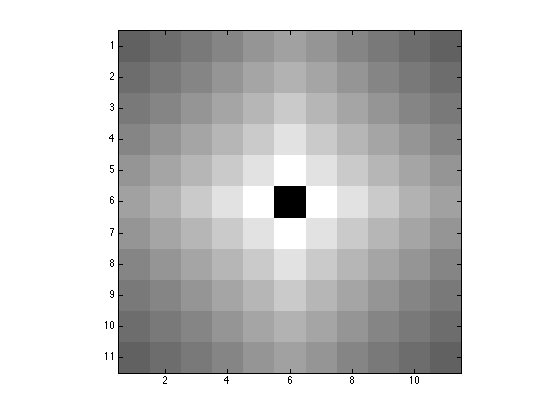
\includegraphics[width=\textwidth]
        {valueIterationColormap.png}}
        \caption{\label{colormapValueIteration} Colormap of the $V$-values  resulting from value iteration for $\theta=0$ and $\gamma = 0.9$. The brighter the color the higher the corresponding $V$-value.}
      \end{figure}

\newpage
\begin{landscape}

\begin{table}[tbp]
\centering
\begin{tabular} {c c c c c c c c c c c c}
 & 0 & 1 & 2 & 3 & 4 & 5 & 6 & 7 & 8 & 9 & 10 \\
0 & 0.000000 & 0.000002 & 0.000011 & 0.000074 & 0.000438 & 0.001730 & 0.000438 & 0.000074 & 0.000011 & 0.000002 & 0.000000\\
1 & 0.000002 & 0.000011 & 0.000075 & 0.000498 & 0.003195 & 0.013773 & 0.003195 & 0.000498 & 0.000075 & 0.000011 & 0.000002\\
2& 0.000011 & 0.000075 & 0.000498 & 0.003443 & 0.021739 & 0.117564 & 0.021739 & 0.003443 & 0.000498 & 0.000075 & 0.000011\\
3 & 0.000074 & 0.000498 & 0.003443 & 0.021739 & 0.166976 & 0.816327 & 0.166976 & 0.021739 & 0.003443 & 0.000498 & 0.000074\\
4 & 0.000438 & 0.003195 & 0.021739 & 0.166976 & 0.816327 & 10.000000 & 0.816327 & 0.166976 & 0.021739 & 0.003195 & 0.000438\\
5 & 0.001730 & 0.013773 & 0.117564 & 0.816327 & 10.000000 & 0.000000 & 10.000000 & 0.816327 & 0.117564 & 0.013773 & 0.001730\\
6 & 0.000438 & 0.003195 & 0.021739 & 0.166976 & 0.816327 & 10.000000 & 0.816327 & 0.166976 & 0.021739 & 0.003195 & 0.000438\\
7 & 0.000074 & 0.000498 & 0.003443 & 0.021739 & 0.166976 & 0.816327 & 0.166976 & 0.021739 & 0.003443 & 0.000498 & 0.000074\\
8 & 0.000011 & 0.000075 & 0.000498 & 0.003443 & 0.021739 & 0.117564 & 0.021739 & 0.003443 & 0.000498 & 0.000075 & 0.000011\\
9 & 0.000002 & 0.000011 & 0.000075 & 0.000498 & 0.003195 & 0.013773 & 0.003195 & 0.000498 & 0.000075 & 0.000011 & 0.000002\\
10 & 0.000000 & 0.000002 & 0.000011 & 0.000074 & 0.000438 & 0.001730 & 0.000438 & 0.000074 & 0.000011 & 0.000002 & 0.000000\\
\end{tabular}\\
\caption{The $V$-values for Value Iteration, with $\gamma$ = 0.1 and the prey at position (5,5). The convergence speed is 20 iterations.}
\label{valueiterationone}
\end{table}

\begin{table}[tbp]
\centering
\begin{tabular} {c c c c c c c c c c c c}
 & 0 & 1 & 2 & 3 & 4 & 5 & 6 & 7 & 8 & 9 & 10 \\
 0 & 0.0267 &  0.0502 &  0.0943 &  0.1768 &  0.3328 &  0.5332 &  0.3328 &  0.1768 &  0.0943 &  0.0502 &  0.0267\\
1 & 0.0502 &  0.0924 &  0.1769 &  0.3390 &  0.6448 &  1.0814 &  0.6448 &  0.3390 &  0.1769 &  0.0924 &  0.0502\\
2 & 0.0943 &  0.1769 &  0.3390 &  0.6498 &  1.2435 &  2.2027 &  1.2435 &  0.6498 &  0.3390 &  0.1769 &  0.0943\\
3 & 0.1768 &  0.3390 &  0.6498 &  1.2435 &  2.3977 &  4.4444 &  2.3977 &  1.2435 &  0.6498 &  0.3390 &  0.1768\\
4 & 0.3328 &  0.6448 &  1.2435 &  2.3977 &  4.4444 & 10.0000 &  4.4444 &  2.3977 &  1.2435 &  0.6448 &  0.3328\\
5 & 0.5332 &  1.0814 &  2.2027 &  4.4444 & 10.0000 &  0.0000 & 10.0000 &  4.4444 &  2.2027 &  1.0814 &  0.5332\\
6 & 0.3328 &  0.6448 &  1.2435 &  2.3977 &  4.4444 & 10.0000 &  4.4444 &  2.3977 &  1.2435 &  0.6448 &  0.3328\\
7 & 0.1768 &  0.3390 &  0.6498 &  1.2435 &  2.3977 &  4.4444 &  2.3977 &  1.2435 &  0.6498 &  0.3390 &  0.1768\\
8 & 0.0943 &  0.1769 &  0.3390 &  0.6498 &  1.2435 &  2.2027 &  1.2435 &  0.6498 &  0.3390 &  0.1769 &  0.0943\\
9 & 0.0502 &  0.0924 &  0.1769 &  0.3390 &  0.6448 &  1.0814 &  0.6448 &  0.3390 &  0.1769 &  0.0924 &  0.0502\\
10 & 0.0267 &  0.0502 &  0.0943 &  0.1768 &  0.3328 &  0.5332 &  0.3328 &  0.1768 &  0.0943 &  0.0502 &  0.0267\\
\end{tabular}\\
\caption{The $V$-values for Value Iteration, with $\gamma$ = 0.5 and the prey at position (5,5). The convergence speed is 28 iterations.}
\label{valueiteration2}
\end{table}

\begin{table}[tbp]
\centering
\begin{tabular} {c c c c c c c c c c c c}
 & 0 & 1 & 2 & 3 & 4 & 5 & 6 & 7 & 8 & 9 & 10 \\
0 &  0.4348 &  0.6065 &  0.8453 &  1.1765 &  1.6463 &  2.1169 &  1.6463 &  1.1765 &  0.8453 &  0.6065 &  0.4348\\
1 &  0.6065 &  0.8328 &  1.1750 &  1.6587 &  2.3345 &  3.0759 &  2.3345 &  1.6587 &  1.1750 &  0.8328 &  0.6065\\
2 &  0.8453 &  1.1750 &  1.6587 &  2.3415 &  3.3044 &  4.4805 &  3.3044 &  2.3415 &  1.6587 &  1.1750 &  0.8453\\
3 &  1.1765 &  1.6587 &  2.3415 &  3.3044 &  4.6737 &  6.5116 &  4.6737 &  3.3044 &  2.3415 &  1.6587 &  1.1765\\
4 &  1.6463 &  2.3345 &  3.3044 &  4.6737 &  6.5116 & 10.0000 &  6.5116 &  4.6737 &  3.3044 &  2.3345 &  1.6463\\
5 &  2.1169 &  3.0759 &  4.4805 &  6.5116 & 10.0000 &  0.0000 & 10.0000 &  6.5116 &  4.4805 &  3.0759 &  2.1169\\
6 &  1.6463 &  2.3345 &  3.3044 &  4.6737 &  6.5116 & 10.0000 &  6.5116 &  4.6737 &  3.3044 &  2.3345 &  1.6463\\
7 &  1.1765 &  1.6587 &  2.3415 &  3.3044 &  4.6737 &  6.5116 &  4.6737 &  3.3044 &  2.3415 &  1.6587 &  1.1765\\
8 &  0.8453 &  1.1750 &  1.6587 &  2.3415 &  3.3044 &  4.4805 &  3.3044 &  2.3415 &  1.6587 &  1.1750 &  0.8453\\
9 &  0.6065 &  0.8328 &  1.1750 &  1.6587 &  2.3345 &  3.0759 &  2.3345 &  1.6587 &  1.1750 &  0.8328 &  0.6065\\
10 &  0.4348 &  0.6065 &  0.8453 &  1.1765 &  1.6463 &  2.1169 &  1.6463 &  1.1765 &  0.8453 &  0.6065 &  0.4348\\
\end{tabular}\\
\caption{The $V$-values for Value Iteration, with $\gamma$ = 0.7 and the prey at position (5,5). The convergence speed is 31 iterations.}
\label{valueiteration3}
\end{table}

\begin{table}[tbp]
\centering
\begin{tabular} {c c c c c c c c c c c c}
 & 0 & 1 & 2 & 3 & 4 & 5 & 6 & 7 & 8 & 9 & 10 \\
0 &  3.8831 &  4.2915 &  4.7417 &  5.2374 &  5.7919 &  6.2513 &  5.7919 &  5.2374 &  4.7417 &  4.2915 &  3.8831\\
1 &  4.2915 &  4.7118 &  5.2281 &  5.8024 &  6.4356 &  6.9973 &  6.4356 &  5.8024 &  5.2281 &  4.7118 &  4.2915\\
2 &  4.7417 &  5.2281 &  5.8024 &  6.4401 &  7.1476 &  7.8390 &  7.1476 &  6.4401 &  5.8024 &  5.2281 &  4.7417\\
3 &  5.2374 &  5.8024 &  6.4401 &  7.1476 &  7.9362 &  8.7805 &  7.9362 &  7.1476 &  6.4401 &  5.8024 &  5.2374\\
4 &  5.7919 &  6.4356 &  7.1476 &  7.9362 &  8.7805 & 10.0000 &  8.7805 &  7.9362 &  7.1476 &  6.4356 &  5.7919\\
5 &  6.2513 &  6.9973 &  7.8390 &  8.7805 & 10.0000 &  0.0000 & 10.0000 &  8.7805 &  7.8390 &  6.9973 &  6.2513\\
6 &  5.7919 &  6.4356 &  7.1476 &  7.9362 &  8.7805 & 10.0000 &  8.7805 &  7.9362 &  7.1476 &  6.4356 &  5.7919\\
7 &  5.2374 &  5.8024 &  6.4401 &  7.1476 &  7.9362 &  8.7805 &  7.9362 &  7.1476 &  6.4401 &  5.8024 &  5.2374\\
8 &  4.7417 &  5.2281 &  5.8024 &  6.4401 &  7.1476 &  7.8390 &  7.1476 &  6.4401 &  5.8024 &  5.2281 &  4.7417\\
9 &  4.2915 &  4.7118 &  5.2281 &  5.8024 &  6.4356 &  6.9973 &  6.4356 &  5.8024 &  5.2281 &  4.7118 &  4.2915\\
10 &  3.8831 &  4.2915 &  4.7417 &  5.2374 &  5.7919 &  6.2513 &  5.7919 &  5.2374 &  4.7417 &  4.2915 &  3.8831\\\end{tabular}\\
\caption{The $V$-values for Value Iteration, with $\gamma$ = 0.9 and the prey at position (5,5). The convergence speed is 34 iterations.}
\label{valueiteration4}
\end{table}


\end{landscape}
\newpage


\subsection{(SC) Policy Iteration}

\newpage
\section{Appendix}
Assignment 1 first \textbf{M}, 100 runs for the random policy predator.\\\\
Timesteps:421\\
Timesteps:831\\
Timesteps:476\\
Timesteps:74\\
Timesteps:537\\
Timesteps:40\\
Timesteps:468\\
Timesteps:465\\
Timesteps:105\\
Timesteps:123\\
Timesteps:227\\
Timesteps:658\\
Timesteps:696\\
Timesteps:153\\
Timesteps:426\\
Timesteps:431\\
Timesteps:24\\
Timesteps:197\\
Timesteps:517\\
Timesteps:313\\
Timesteps:492\\
Timesteps:213\\
Timesteps:457\\
Timesteps:392\\
Timesteps:47\\
Timesteps:178\\
Timesteps:459\\
Timesteps:624\\
Timesteps:881\\
Timesteps:100\\
Timesteps:244\\
Timesteps:127\\
Timesteps:213\\
Timesteps:145\\
Timesteps:45\\
Timesteps:301\\
Timesteps:628\\
Timesteps:248\\
Timesteps:88\\
Timesteps:123\\
Timesteps:82\\
Timesteps:206\\
Timesteps:181\\
Timesteps:771\\
Timesteps:114\\
Timesteps:238\\
Timesteps:118\\
Timesteps:67\\
Timesteps:41\\
Timesteps:662\\
Timesteps:27\\
Timesteps:73\\
Timesteps:217\\
Timesteps:269\\
Timesteps:382\\
Timesteps:60\\
Timesteps:205\\
Timesteps:64\\
Timesteps:133\\
Timesteps:232\\
Timesteps:148\\
Timesteps:504\\
Timesteps:113\\
Timesteps:316\\
Timesteps:151\\
Timesteps:178\\
Timesteps:53\\
Timesteps:526\\
Timesteps:150\\
Timesteps:690\\
Timesteps:490\\
Timesteps:116\\
Timesteps:288\\
Timesteps:79\\
Timesteps:163\\
Timesteps:266\\
Timesteps:566\\
Timesteps:1194\\
Timesteps:133\\
Timesteps:690\\
Timesteps:136\\
Timesteps:121\\
Timesteps:123\\
Timesteps:492\\
Timesteps:288\\
Timesteps:185\\
Timesteps:19\\
Timesteps:78\\
Timesteps:250\\
Timesteps:42\\
Timesteps:268\\
Timesteps:190\\
Timesteps:231\\
Timesteps:393\\
Timesteps:338\\
Timesteps:100\\
Timesteps:49\\
Timesteps:653\\
Timesteps:1173\\
Timesteps:421\\
Average timesteps over 100 trials: 296.93\\
Standard deviation over 100 trials: 244.54689754728025\\

\end{document}
